\subsection{Glyph: \glyph{Dissociation}}
\label{sec:dissociation}

The \glyph{dissociation} of an \glyph{EPN} into one or more \glyph{EPNs} represents the rupture of a non-covalent binding between the biological entities represented by those \glyph{EPNs}.

\begin{glyphDescription}

\glyphSboTerm
SBO:0000180 ! dissociation


\glyphIncoming
One \glyph{consumption} arc (\sect{consumption}), zero or more \glyph{modulation} arcs (\sect{modulations}).



\glyphOutgoing
One or more \glyph{production} arcs (\sect{production}).


\glyphContainer
A \glyph{process} is represented by a circular shape containing another concentric circle.
The shape is linked to two ports, that are small arcs attached to the centres of opposite sides of the shape, as shown in \fig{dissociation}.
The incoming \glyph{consumption} (\sect{consumption}) and outgoing \glyph{production} (\sect{production}) arcs are linked to the extremities of those ports.

The \glyph{modulation arcs} (\sect{modulations}) point to the other two sides of the shape.

\glyphLabel
None.

\glyphAux
None.

\end{glyphDescription}

\begin{figure}[H]
  \centering
  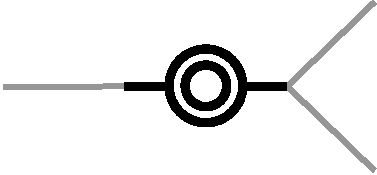
\includegraphics{images/dissociation}
  \caption{The \PD glyph for \glyph{dissociation}.}
  \label{fig:dissociation}
\end{figure}

The example in \fig{dissoc-ribo} illustrates the dissociation of the small and large ribosomal subunits from a messenger RNA.

\begin{figure}[H]
  \centering
  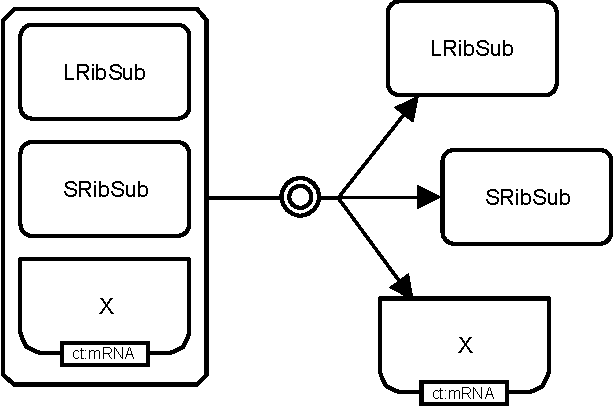
\includegraphics[scale = 0.8]{examples/dissociation-ribosome}
  \caption{Dissociation of the small and large ribosomal subunits from a messenger RNA.}
  \label{fig:dissoc-ribo}
\end{figure}
